\usepackage{ifthen}

% Define an agenda item
%
% Arguments:
% 1: Identifier of the agenda item, should be all lower-case
% 2: Type of the agenda item: lecture or lab
% 3: English title of the agenda item
% 4: English full description of the agenda item
% 5: French title of the agenda item
% 6: French full description of the agenda item
\newcommand\defagendaitem[6]{
  \ifthenelse{\equal{\agendalanguage}{french}}{
    \expandafter\def\csname #1@#2@title\endcsname {#5}
    \expandafter\def\csname #1@#2@contents\endcsname {#6}
  }{
    \expandafter\def\csname #1@#2@title\endcsname {#3}
    \expandafter\def\csname #1@#2@contents\endcsname {#4}
  }
}

% Show/render an agenda item
%
% Arguments:
% 1: Identifier of the agenda item, as defined by \defagendaitem
% 2: Type of the agenda item: lecture or lab
\newcommand\showagendaitem[2]{
  \ifthenelse{\boolean{hlineneeded}}{\\\hline}{\setboolean{hlineneeded}{true}}
    \ifthenelse{\equal{\agendalanguage}{french}}{
      \ifthenelse{\equal{#2}{lecture}}
      {Cours &}
      {
        \ifthenelse{\equal{#2}{lab}}{
          \ifthenelse{\equal{\trainingtype}{online}}{Démo &}{TP &}
        }
        {}
      }
    }{
      \ifthenelse{\equal{#2}{lecture}}
      {Lecture &}
      {
        \ifthenelse{\equal{#2}{lab}}{
          \ifthenelse{\equal{\trainingtype}{online}}{Demo &}{Lab &}
        }
        {}
      }
    }
    \csname #1@#2@title\endcsname &
    \vspace{-8pt}
    \csname #1@#2@contents\endcsname
}

% Define a board
%
% Arguments:
% 1: Identifier for the board, must be all lower-case
% 2: English title
% 3: English full description
% 4: French title
% 5: French full description
% 6: Board picture
\newcommand\defboard[6]{
  \ifthenelse{\equal{\agendalanguage}{french}}{
    \expandafter\def\csname #1@title\endcsname {#4}
    \expandafter\def\csname #1@contents\endcsname {#5}
  }{
    \expandafter\def\csname #1@title\endcsname {#2}
    \expandafter\def\csname #1@contents\endcsname {#3}
  }
  \expandafter\def\csname #1@image\endcsname {#6}
}

% Show/render a board
%
% Arguments:
% 1: Identifier of the board, as defined by \defboard
\newcommand\showboarditem[1]{
  \begin{tabularx}{\textwidth}{p{7cm}p{11cm}}
    \arrayrulecolor{blorange}
    \hline
    \multicolumn{1}{l}{\textbf{\textcolor{blorange}{\large \csname #1@title\endcsname}}} & \\
    \hline
    \arrayrulecolor{gray}
    \csname #1@contents\endcsname &
    \csname #1@image\endcsname \\
  \end{tabularx}
}

% Start an agenda by finding
% out if it is a morning or an
% afternoon if the training
% takes place on site
%
% Arguments:
% 1: Number of the half-day
\newcommand\showagendaday[1]{
  \arrayrulecolor{blorange}
  \\\hline
  \multicolumn{3}{l}{%
    \textbf{\textcolor{blorange}{\large\hspace{-1.5em}
      \ifthenelse{\equal{\trainingtype}{online}}{
        \showonlineagendaday{#1}
      }{
        \pgfmathparse{int(mod(#1, 2))}
        \ifnum\pgfmathresult=1
          \pgfmathparse{int((#1 + 1) / 2)}
          \showonsiteagendaday{\pgfmathresult}{morning}
        \else
          \pgfmathparse{int(#1 / 2)}
          \showonsiteagendaday{\pgfmathresult}{afternoon}
        \fi
      }
    }}
  } \\
  \hline
  \setboolean{hlineneeded}{false}
  \arrayrulecolor{gray}
}

% Start an online agenda half-day
%
% Arguments:
% 1: Number of the half-day
\newcommand\showonlineagendaday[1]{
  \ifthenelse{\equal{\agendalanguage}{french}}{
    Demi-journée #1
  }{
    Half day #1
  }
}

% Start an on-site agenda half-day
%
% Arguments:
% 1: Number of the day
% 2: "morning" or "afternoon"
\newcommand\showonsiteagendaday[2]{
  \ifthenelse{\equal{\agendalanguage}{french}}{
    \ifthenelse{\equal{#2}{morning}}{
      Jour #1 - Matin
    }{
      Jour #1 - Après-midi
    }
  }{
    \ifthenelse{\equal{#2}{morning}}{
      Day #1 - Morning
    }{
      Day #1 - Afternoon
    }
  }
}

\defboard
{stm32mp1}
{STM32MP1 Discovery Kit}
{
  One of these Discovery Kits from STMicroelectronics: {\bf
  STM32MP157A-DK1}, {\bf STM32MP157D-DK1}, {\bf STM32MP157C-DK2} or
  {\bf STM32MP157F-DK2}
  \begin{itemize}
  \item STM32MP157, dual Cortex-A7 processor from STMicroelectronics
  \item USB powered
  \item 512 MB DDR3L RAM
  \item Gigabit Ethernet port
  \item 4 USB 2.0 host ports
  \item 1 USB-C OTG port
  \item 1 Micro SD slot
  \item On-board ST-LINK/V2-1 debugger
  \item Arduino compatible headers
  \item Audio codec, buttons, LEDs
  \item LCD touchscreen (DK2 kits only)
  \vspace{-0.7cm}
  \end{itemize}
}
{Plateforme STM32MP1}
{
  Une de ces cartes de STMicroelectronics : {\bf
  STM32MP157A-DK1}, {\bf STM32MP157D-DK1}, {\bf STM32MP157C-DK2} ou
  {\bf STM32MP157F-DK2}
  \begin{itemize}
  \item Processeur STM32MP157, double Cortex-A7, de STMicroelectronics
  \item Alimentée par USB
  \item 512 Mo DDR3L RAM
  \item Port Gigabit Ethernet port
  \item 4 ports hôte USB 2.0
  \item 1 port USB-C OTG
  \item 1 connecteur Micro SD
  \item Debugger ST-LINK/V2-1 sur la carte
  \item Connecteurs compatibles Arduino Uno v3
  \item Codec audio
  \item Divers : boutons, LEDs
  \item Écran LCD tactile (uniquement sur cartes DK2)
  \vspace{-0.7cm}
  \end{itemize}
}
{
  \begin{center}
    \includegraphics[width=5cm]{../slides/discovery-board-dk1/discovery-board-dk1.png}
  \end{center}
}

\defagendaitem
{qna}
{misc}
{Questions and Answers}
{
  \begin{itemize}
  \item Questions and answers with the audience about the course topics
  \item Extra presentations if time is left, according what most
        participants are interested in.
  \end{itemize}
}
{Questions / réponses}
{
  \begin{itemize}
  \item Questions et réponses avec les participants à propos des sujets abordés.
  \item Présentations supplémentaires s'il reste du temps, en fonction des demandes
        de la majorité des participants.
  \end{itemize}
}


\defboard
{beagleboneblack}
{BeagleBone Black}
{
  {\bf BeagleBone Black} or {\bf BeagleBone Black Wireless} board
  \begin{itemize}
  \item An ARM AM335x (single Cortex-A8) processor from Texas
    Instruments
  \item USB powered
  \item 512 MB of RAM
  \item 2 or 4 GB of on-board eMMC storage
  \item USB host and device
  \item HDMI output
  \item 2 x 46 pins headers, to access UARTs, SPI buses, I2C buses
    and more.
  \item Ethernet or WiFi
  \end{itemize}
  \vspace{-0.7cm}
}
{BeagleBone Black}
{
  Carte {\bf BeagleBone Black} ou {\bf BeagleBone Black Wireless}
  \begin{itemize}
  \item Un processeur ARM AM335x de Texas Instruments (à base de
    Cortex-A8), avec accélération 3D, etc.
  \item 512 Mo de RAM
  \item 2 ou 4 Go de stockage eMMC
  \item USB hôte et device
  \item Sortie HDMI
  \item Connecteurs à 2 x 46 broches, pour accéder aux UARTs, aux bus
    SPI, aux bus I2C, et à d'autres entrées/sorties du processeur.
  \item Ethernet ou WiFi
  \vspace{-0.7cm}
  \end{itemize}
}
{
  \begin{center}
    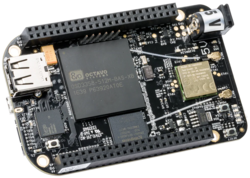
\includegraphics[width=5cm]{../slides/beagleboneblack-board/beagleboneblack_sd.png}
  \end{center}
}

\defboard
{beagleplay}
{BeaglePlay}
{
  {\bf BeaglePlay} board
  \begin{itemize}
    \item Texas Instruments AM625x (4xARM Cortex-A53 CPU)
    \item SoC with 3D acceleration, integrated MCU and many other peripherals.
    \item 2 GB of RAM
    \item 16 GB of on-board eMMC storage
    \item USB host and USB device, microSD, HDMI
    \item 2.4 and 5 GHz WiFi, Bluetooth and also Ethernet
    \item 1 MicroBus Header (SPI, I2C, UART, ...), OLDI and CSI connector.
  \vspace{-0.7cm}
  \end{itemize}
}
{BeaglePlay}
{
  Carte {\bf BeaglePlay}
  \begin{itemize}
    \item SoC Texas Instruments AM625x (CPU 4xARM Cortex-A53)
    \item SoC avec accélération 3D, MCU intégré et de nombreux autres périphériques.
    \item 2 GB de RAM
    \item 16 Go de stockage eMMC
    \item USB hôte et device, microSD, HDMI
    \item WiFi 2.4 and 5 GHz, Bluetooth et aussi Ethernet
    \item 1 Header MicroBus (SPI, I2C, UART, ...), connecteurs OLDI et CSI.
  \vspace{-0.7cm}
  \end{itemize}
}
{
  \begin{center}
    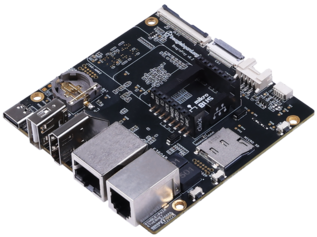
\includegraphics[width=5cm]{../slides/beagleplay-board/beagleplay_sd.png}
  \end{center}
}


\def \training{yocto}

% Title
\ifthenelse{\equal{\agendalanguage}{french}}{
  \def \trainingtitle{Formation développement Linux embarqué
  \newline avec Yocto Project et OpenEmbedded}
}{
  \def \trainingtitle{Yocto Project and OpenEmbedded development training}
}

% Duration
\ifthenelse{\equal{\trainingtype}{online}}{
  \def \trainingduration{4}
}{
  \def \trainingduration{3}
}

\def \trainingicon{common/flaticon-yocto-training.png}

% Training objectives
\ifthenelse{\equal{\agendalanguage}{french}}{
  \def \traininggoals{
    \begin{itemize}
    \item Être capable de comprendre le rôle et le principe d'un build
      system Linux embarqué, et comparer Yocto Project/OpenEmbedded aux
      autres outils offrant des fonctionnalités similaires.
    \item Être capable de configurer et de réaliser la compilation d'un
      système Linux embarqué simple avec Yocto, et d'installer le
      résultat sur une plateforme embarquée.
    \item Être capable d'écrire ou d'étendre des recettes de paquets,
      pour vos propres paquets ou personnalisations.
    \item Être capable d'utiliser des {\em layers} de recettes
      existants, et de créer votre propre nouveau {\em layer}.
    \item Être capable d'intégrer le support pour votre carte embarqué
      dans un {\em layer BSP}.
    \item Être capable de créer des images personnalisées.
    \item Être capable d'utiliser le SDK du Yocto Project pour développer
      des applications.
    \item Être capable d'utiliser devtool pour développer une recette.
    \end{itemize}
  }
}{
  \def \traininggoals{
    \begin{itemize}
    \item Be able to understand the role and principle of an embedded
      Linux build system, and compare Yocto Project/OpenEmbedded to
      other tools offering similar functionality.
    \item Be able to configure and build basic embedded Linux system
      with Yocto, and install the result on an embedded platform.
    \item Be able to write and extend recipes, for your own packages or
      customizations.
    \item Be able to use existing layers of recipes, and create your own
      new layers.
    \item Be able to integrate support for your own embedded board into
      a BSP layer.
    \item Be able to create custom images.
    \item Be able to use the Yocto Project SDK to develop applications.
    \item Be able to use devtool to generate and modify recipes.
    \end{itemize}
  }
}

\def \feshowboards{
    \ifthenelse{\equal{\agendalanguage}{french}}{
      \section{Plateformes matérielle pour les travaux pratiques}
    }{
      \section{Hardware platform for practical labs}
    }

  \showboarditem{stm32mp1}
  \showboarditem{beagleboneblack}
  \showboarditem{beagleplay}
  \newpage
}

% Training prerequisites
\def \trainingprerequisites{
  \begin{itemize}
    \prerequisitecommandline
    \prerequisiteembeddedlinux
    \prerequisiteenglish
  \end{itemize}
}

% Training audience
\ifthenelse{\equal{\agendalanguage}{french}}{
  \def \trainingaudience{
    Sociétés et ingénieurs intéressés par l'utilisation de Yocto
    Project pour construire leur système Linux embarqué.
  }
}{
  \def \trainingaudience{
    Companies and engineers interested in using the Yocto Project to
    build their embedded Linux system.
  }
}

\ifthenelse{\isundefined{\traininglanguages}}{
  \ifthenelse{\equal{\agendalanguage}{french}}{
    \def \traininglanguages{
      \begin{tabular}{p{2.2cm} @{\hskip 0.2cm}p{5cm}}
	Transparents & Anglais \\
	\\
	Présentation & Français \\
	 & Anglais \\
	 & Italien \\
      \end{tabular}
    }
  }{
    \def \traininglanguages{
      \begin{tabular}{p{2.2cm} @{\hskip 0.2cm}p{5cm}}
	Materials & English \\
	\\
	Oral Lecture & English \\
	 & French \\
	 & Italian \\
      \end{tabular}
    }
  }
}

% Time ratio
\def \onsitelecturetimeratio{40}
\def \onsitelabtimeratio{60}

% Agenda items

\defagendaitem
{intro}
{lecture}
{Introduction to embedded Linux build systems}
{
  \begin{itemize}
  \item Overview of an embedded Linux system architecture
  \item Methods to build a root filesystem image
  \item Usefulness of build systems
  \end{itemize}
}
{Introduction aux outils de compilation de systèmes Linux embarqué}
{
  \begin{itemize}
  \item Vue d'ensemble de l'architecture d'un système Linux embarqué
  \item Méthodes pour compiler un système de fichiers
  \item Utilité des outils de compilation
  \end{itemize}
}

\defagendaitem
{overview}
{lecture}
{Overview of the Yocto Project and the Poky reference system}
{
  \begin{itemize}
  \item Introduction to the Yocto / OpenEmbedded build system and its lexicon
  \item Overview of the Poky reference system
  \end{itemize}
}
{Vue d'ensemble de Yocto Project et du système de référence Poky}
{
  \begin{itemize}
  \item Organisation des sources du projet
  \item Création d'un système de fichiers avec Yocto Project
  \end{itemize}
}

\defagendaitem
{overview}
{lecture}
{Yocto Project and Poky reference system overview}
{
  \begin{itemize}
  \item Introduction to the Yocto / OpenEmbedded build system and its lexicon
  \item Overview of the Poky reference system
  \end{itemize}
}
{Vue d'ensemble de Yocto Project et du système de référence Poky}
{
  \begin{itemize}
  \item Présentation de l'outil de compilation Yocto / OpenEmbedded et de sa terminologie.
  \item Vue d'ensemble du système de référence Poky
  \end{itemize}
}

\defagendaitem
{usingbasics}
{lecture}
{Using Yocto Project - basics}
{
  \begin{itemize}
  \item Setting up the build directory and environment
  \item Configuring the build system
  \item Building a root filesystem image
  \item Organization of the build output
  \end{itemize}
}
{Bases de l'utilisation de Yocto Project}
{
  \begin{itemize}
  \item Mise en place du répertoire de travail et de l'environnement
  \item Configuration de l'outil de compilation
  \item Compilation de l'image d'un système de fichiers racine
  \item Structure des fichiers générés
  \end{itemize}
}

\defagendaitem
{firstbuild}
{lab}
{First Yocto Project build}
{
  \begin{itemize}
  \item Downloading the Poky reference build system
  \item Configuring the build system
  \item Building a system image
 \end{itemize}
}
{1\textsuperscript{ère} compilation avec Yocto Project}
{
  \begin{itemize}
  \item Téléchargement du système de référence Poky
  \item Configuration de l'outil de compilation
  \item Compilation d'une image système
 \end{itemize}
}

\defagendaitem
{flashingbooting}
{lab}
{Flashing and booting}
{
  \begin{itemize}
  \item Flashing and booting the image on the board
  \end{itemize}
}
{Flasher et booter}
{
  \begin{itemize}
  \item Flasher et booter l'image du système sur la carte
  \end{itemize}
}

\defagendaitem
{usingadvanced}
{lecture}
{Using Yocto Project - advanced usage}
{
  \begin{itemize}
  \item Variable assignment, operators and overrides
  \item Package variants and package selection
  \item bitbake command line options
  \end{itemize}
}
{Utilisation de Yocto Project - Utilisation avancée}
{
  \begin{itemize}
  \item Assignation des variables, opérateurs et surcharge
  \item Paquetages: variantes de paquetages
  \item Options de la commande bitbake
  \end{itemize}
}

\defagendaitem
{nfsconfiguring}
{lab}
{Using NFS and configuring the build}
{
  \begin{itemize}
  \item Configuring the board to boot over NFS
  \item Add a package to the root filesystem
  \item Learn how to use the \code{PREFERRED_PROVIDER} mechanism
  \item Get familiar with the bitbake command line options
  \end{itemize}
}
{Utilisation de NFS et configuration de la compilation}
{
  \begin{itemize}
  \item Configurer la carte pour démarrer via NFS
  \item Rajouter un paquetage au système de fichiers racine
  \item Apprendre à utiliser le mécanisme \code{PREFERRED_PROVIDER}
  \item Se familiariser avec les options de la commande bitbake
  \end{itemize}
}

\defagendaitem
{writingrecipesbasics}
{lecture}
{Writing recipes - basics}
{
  \begin{itemize}
  \item Recipes: overview
  \item Recipe file organization
  \item Applying patches
  \item Recipe examples
  \end{itemize}
}
{Écriture de recettes - Fonctionnalités de base}
{
  \begin{itemize}
  \item Recettes: vue d'ensemble
  \item Organisation d'un fichier de recette
  \item Application de patches
  \item Exemples de recettes
  \end{itemize}
}

\defagendaitem
{appcompilation}
{lab}
{Adding an application to the build}
{
  \begin{itemize}
  \item Writing a recipe for {\em ninvaders}
  \item Troubleshooting the recipe
  \item Troubleshooting cross-compilation issues
  \item Adding {\em ninvaders} to the final image
  \end{itemize}
}
{Ajouter la compilation d'une application}
{
  \begin{itemize}
  \item Création d'une recette pour {\em ninvaders}
  \item Résolution de problèmes liés à la recette
  \item Résolution de problèmes liés à la compilation croisée
  \item Ajout d'{\em ninvaders} à l'image finale
  \end{itemize}
}

\defagendaitem
{writingrecipesadvanced}
{lecture}
{Writing recipes - advanced features}
{
  \begin{itemize}
  \item Extending and overriding recipes
  \item Virtual packages
  \item Learn about classes
  \item BitBake file inclusions
  \item Debugging recipes
  \item Configuring BitBake network usage
  \end{itemize}
}
{Écriture de recettes - Fonctionnalités avancées}
{
  \begin{itemize}
  \item Extension et redéfinition de recettes
  \item Paquetages virtuels
  \item Familiarisation avec les classes
  \item Inclusion d'exemples avec BitBake
  \item Mise au point des recettes
  \item Configuration de l'utilisation du réseau par BitBake
  \end{itemize}
}

\defagendaitem
{layers}
{lecture}
{Layers}
{
  \begin{itemize}
  \item What layers are
  \item Where to find layers
  \item Creating a layer
  \end{itemize}
}
{Layers}
{
  \begin{itemize}
  \item Ce que sont les {\em layers}
  \item Où trouver les {\em layers}
  \item Création d'un {\em layer}
  \end{itemize}
}

\defagendaitem
{writinglayer}
{lab}
{Writing a layer}
{
  \begin{itemize}
  \item Learn how to write a layer
  \item Add the layer to the build
  \item Move {\em ninvaders} to the new layer
  \end{itemize}
}
{Écriture d'un layer}
{
  \begin{itemize}
  \item Apprendre à écrire un {\em layer}
  \item Ajouter le {\em layer} à la compilation
  \item Inclure {\em ninvaders} dans le nouveau {\em layer}
  \end{itemize}
}

\defagendaitem
{extendrecipe}
{lab}
{Extend a recipe}
{
  \begin{itemize}
  \item Extend the kernel recipe to add patches
  \item Configure the kernel to compile the nunchuk driver
  \item Edit the ninvaders recipe to add patches
  \item Play {\em ninvaders}
  \end{itemize}
}
{Étendre une recette}
{
  \begin{itemize}
  \item Étendre la recette pour le noyau pour rajouter des patches
  \item Configurer le noyau pour compiler le pilote du nunchuk
  \item Modifier la recette ninvaders pour rajouter des patches
  \item Jouer avec {\em ninvaders}
  \end{itemize}
}

\defagendaitem
{writingbsp}
{lecture}
{Writing a BSP}
{
  \begin{itemize}
  \item Introduction to BSP layers
  \item Adding a new machine
  \item Bootloader configuration
  \item Linux: the kernel bbclass and the linux-yocto recipe
  \end{itemize}
}
{Écriture d'un BSP}
{
  \begin{itemize}
  \item Introduction aux layers BSP
  \item Ajout d'une nouvelle machine
  \item Configuration du chargeur de démarrage
  \item Linux : la classe kernel.bbclass et la recette linux-yocto
  \end{itemize}
}

\defagendaitem
{kernelchanges}
{lab}
{Create a custom machine configuration}
{
  \begin{itemize}
  \item Create a new machine configuration
  \item Build an image for the new machine
  \end{itemize}
}
{Création d'une configuration spécifique pour une machine}
{
  \begin{itemize}
  \item Types d'images
  \item Écriture et utilisation de groupes de paquetages
  \end{itemize}
}

\defagendaitem
{distrolayer}
{lecture}
{Distro layers}
{
  \begin{itemize}
  \item Distro configuration
  \item Distro layers
  \end{itemize}
}
{Création d'une image sur mesure}
{
  \begin{itemize}
  \item Rajouter une recette de base pour une image
  \item Sélectionner les fonctionnalités et les paquetages de l'image
  \item Ajouter un groupe de paquetages sur mesure
  \item Ajouter une variante d'image pour le débogage
  \end{itemize}
}

\defagendaitem
{image}
{lecture}
{Images}
{
  \begin{itemize}
  \item Writing an image recipe
  \item Image types
  \item Writing and using package groups recipes
  \end{itemize}
}
{Images}
{
  \begin{itemize}
  \item Écriture d’une recette d’image
  \item Types d’images
  \item Écriture et utilisation de groupes de paquetages
  \end{itemize}
}

\defagendaitem
{image}
{lab}
{Create a custom image}
{
  \begin{itemize}
  \item Add a basic image recipe
  \item Select the image capabilities and packages
  \item Add a custom package group
  \item Add an image variant for debugging
  \end{itemize}
}
{Création d'une image sur mesure}
{
  \begin{itemize}
  \item Écrire une recette d'image personnalisée
  \item Ajouter {\em ninvaders} à l'image sur mesure
  \end{itemize}
}

\defagendaitem
{writingrecipesgoingfurther}
{lecture}
{Writing recipes - going further}
{
  \begin{itemize}
  \item The per-recipe sysroot
  \item Using Python code in metadata
  \item Variable flags
  \item Packages features and PACKAGECONFIG
  \item Conditional features
  \item Package splitting
  \item Dependencies in detail
  \end{itemize}
}
{Écriture de recettes - Pour aller plus loin}
{
  \begin{itemize}
  \item Le sysroot de chaque recette
  \item Utilisation de code Python code dans les méta-données
  \item Drapeaux de variables
  \item Fonctionnalités de paquetages et PACKAGECONFIG
  \item Fonctionnalités conditionnelles
  \item Découpage de paquetages
  \end{itemize}
}

\defagendaitem
{licensing}
{lecture}
{Licensing}
{
  \begin{itemize}
  \item Managing open source licenses
  \end{itemize}
}
{Licences}
{
  \begin{itemize}
  \item Gestion de licences open source
  \end{itemize}
}

\defagendaitem
{sdk}
{lecture}
{The Yocto Project SDK}
{
  \begin{itemize}
  \item Goals of the SDK
  \item Building and customizing an SDK
  \item Using the Yocto Project SDK
  \end{itemize}
}
{SDK pour le projet Yocto}
{
  \begin{itemize}
  \item Objectifs du SDK
  \item Compilation et personnalisation d'un SDK
  \item Utilisation d'un SDK pour le projet Yocto
  \end{itemize}
}

\defagendaitem
{sdk}
{lab}
{Develop your application in the Poky SDK}
{
  \begin{itemize}
  \item Building an SDK
  \item Using the Yocto Project SDK
  \end{itemize}
}
{Développement d'une application au moyen du SDK de Poky}
{
  \begin{itemize}
  \item Construction d'un SDK
  \item Utilisation du SDK de Yocto Project
  \end{itemize}
}

\defagendaitem
{devtool}
{lecture}
{Devtool}
{
  \begin{itemize}
  \item About devtool
  \item Devtool use cases
  \end{itemize}
}
{Devtool}
{
  \begin{itemize}
  \item Présentation devtool
  \item Cas d'utilisation de devtool
  \end{itemize}
}

\defagendaitem
{devtool}
{lab}
{Using devtool}
{
  \begin{itemize}
  \item Generate a new recipe
  \item Modify a recipe to add a new patch
  \item Upgrade a recipe to a newer version
  \end{itemize}
}
{Utilisation de devtool}
{
  \begin{itemize}
  \item Création d'une nouvelle recette
  \item Modification d'une recette pour ajouter un nouveau patch
  \item Mettre à jour une recette pour prendre en charge une nouvelle version
  \end{itemize}
}

\defagendaitem
{automatinglayermanagement}
{lecture}
{Automating layer management}
{
  \begin{itemize}
  \item Automating layer management
  \end{itemize}
}
{Gestion automatique de layers}
{
  \begin{itemize}
  \item Gestion automatique de layers
  \end{itemize}
}

\defagendaitem
{runtimepackagemanagement}
{lecture}
{Runtime Package Management}
{
  \begin{itemize}
  \item Introduction to runtime package management
  \item Build configuration
  \item Package server configuration
  \item Target configuration
  \end{itemize}
}
{Gestion de paquetages à l'exécution}
{
  \begin{itemize}
  \item Introduction à la gestion de paquetages à l'exécution
  \item Configuration de la compilation
  \item Configuration d'une serveur de paquetages
  \item Configuration de la machine cible
  \end{itemize}
}

\def \onlineagenda {
  \ifthenelse{\equal{\agendalanguage}{french}}{
    \section{Programme de la formation}
  }{
    \section{Training Schedule}
  }
  \begin{tabularx}{\textwidth}{p{2cm}p{5cm}p{11cm}}
  \showagendaday{1}
  \showagendaitem{intro}{lecture}
  \showagendaitem{overview}{lecture}
  \showagendaitem{usingbasics}{lecture}
  \showagendaitem{firstbuild}{lab}
  \showagendaitem{flashingbooting}{lab}
  \showagendaday{2}
  \showagendaitem{usingadvanced}{lecture}
  \showagendaitem{nfsconfiguring}{lab}
  \showagendaitem{writingrecipesbasics}{lecture}
  \showagendaitem{appcompilation}{lab}
  \showagendaitem{writingrecipesadvanced}{lecture}
  \showagendaday{3}
  \showagendaitem{layers}{lecture}
  \showagendaitem{writinglayer}{lab}
  \showagendaitem{extendrecipe}{lab}
  \showagendaitem{writingbsp}{lecture}
  \showagendaitem{kernelchanges}{lab}
  \showagendaitem{distrolayer}{lecture}
  \showagendaday{4}
  \showagendaitem{image}{lecture}
  \showagendaitem{image}{lab}
  \showagendaitem{writingrecipesgoingfurther}{lecture}
  \showagendaitem{licensing}{lecture}
  \showagendaitem{sdk}{lecture}
  \showagendaitem{sdk}{lab}
  \showagendaitem{devtool}{lecture}
  \showagendaitem{devtool}{lab}
  \showagendaitem{automatinglayermanagement}{lecture}
  \showagendaitem{runtimepackagemanagement}{lecture}
  \showagendaitem{qna}{misc}
  \end{tabularx}
}

\def \onsiteagenda {
  \ifthenelse{\equal{\agendalanguage}{french}}{
    \section{Programme de la formation}
  }{
    \section{Training Schedule}
  }
  \begin{tabularx}{\textwidth}{p{2cm}p{5cm}p{11cm}}
  \showagendaday{1}
  \showagendaitem{intro}{lecture}
  \showagendaitem{overview}{lecture}
  \showagendaitem{usingbasics}{lecture}
  \showagendaitem{firstbuild}{lab}
  \showagendaday{2}
  \showagendaitem{flashingbooting}{lab}
  \showagendaitem{usingadvanced}{lecture}
  \showagendaitem{nfsconfiguring}{lab}
  \showagendaday{3}
  \showagendaitem{writingrecipesbasics}{lecture}
  \showagendaitem{appcompilation}{lab}
  \showagendaitem{writingrecipesadvanced}{lecture}
  \showagendaday{4}
  \showagendaitem{layers}{lecture}
  \showagendaitem{writinglayer}{lab}
  \showagendaday{5}
  \showagendaitem{extendrecipe}{lab}
  \showagendaitem{writingbsp}{lecture}
  \showagendaitem{kernelchanges}{lab}
  \showagendaitem{distrolayer}{lecture}
  \showagendaday{6}
  \showagendaitem{image}{lecture}
  \showagendaitem{image}{lab}
  \showagendaitem{writingrecipesgoingfurther}{lecture}
  \showagendaitem{licensing}{lecture}
  \showagendaitem{sdk}{lecture}
  \showagendaitem{sdk}{lab}
  \showagendaitem{devtool}{lecture}
  \showagendaitem{devtool}{lab}
  \showagendaitem{automatinglayermanagement}{lecture}
  \showagendaitem{runtimepackagemanagement}{lecture}
  \end{tabularx}
}
